\documentclass[
  notitle]{jss}

\usepackage[utf8]{inputenc}

\providecommand{\tightlist}{%
  \setlength{\itemsep}{0pt}\setlength{\parskip}{0pt}}

\author{
Drago Plecko\\ETH Zürich \And Nicolas Bennett\\ETH Zürich \And Nicolai Meinshausen\\ETH Zürich
}
\title{\pkg{fairadapt}: Causal Reasoning for Fair Data Pre-processing}

\Plainauthor{Drago Plecko, Nicolas Bennett, Nicolai Meinshausen}
\Plaintitle{fairadapt: Causal Reasoning for Fair Data Pre-processing}
\Shorttitle{\pkg{fairadapt}: Fair Data Adaptation}

\Abstract{
Machine learning algorithms are useful for various predictions tasks,
but they can also learn how to discriminate, based on gender, race or
some other sensitive attribute. This realization gave rise to the field
of fair machine learning, which aims to measure and mitigate such
algorithmic bias. This manuscript describes the implementation of the
\pkg{fairadapt} R-package, a causal inference pre-processing method,
which, using the causal graphical model, answers hypothetical questions
of the form ``What would my salary have been, had I been of a different
gender/race?''. Such counterfactual reasoning can help eliminate
discrimination and help justify fair decisions.
}

\Keywords{algorithmic fairness, causal inference, machine learning}
\Plainkeywords{algorithmic fairness, causal inference, machine learning}

%% publication information
%% \Volume{50}
%% \Issue{9}
%% \Month{June}
%% \Year{2012}
%% \Submitdate{}
%% \Acceptdate{2012-06-04}

\Address{
    Drago Plecko\\
    ETH Zürich\\
    Seminar for Statistics Rämistrasse 101 CH-8092 Zurich\\
  E-mail: \email{drago.plecko@stat.math.ethz.ch}\\
  
      Nicolas Bennett\\
    ETH Zürich\\
    Seminar for Statistics Rämistrasse 101 CH-8092 Zurich\\
  E-mail: \email{nicolas.bennett@stat.math.ethz.ch}\\
  
      Nicolai Meinshausen\\
    ETH Zürich\\
    Seminar for Statistics Rämistrasse 101 CH-8092 Zurich\\
  E-mail: \email{meinshausen@stat.math.ethz.ch}\\
  
  }

% Pandoc citation processing

% Pandoc header

\usepackage{amsmath} \usepackage{tikz} \usepackage{algorithm2e} \usepackage{bbm} \usepackage{pgfplots} \usepackage{array} \usepackage{enumerate}

\usetikzlibrary{arrows.meta} \newtheorem{definition}{Definition}
\newcommand{\pa}{\mathrm{pa}} \newcommand{\Pa}{\mathrm{Pa}}
\newcommand{\de}{\mathrm{de}} \newcommand{\ch}{\mathrm{ch}}
\newcommand{\an}{\mathrm{an}}

\newcommand{\drago}[1]{{\color{red} Drago: {#1}}} \newcommand{\pr}{\mathbbm{P}} \newcommand{\ex}{\mathbbm{E}} \renewcommand{\tilde}[1]{ {#1}^{(fp)}} \def\ci{{\perp\!\!\!\perp}} \pgfmathdeclarefunction{gauss}{2}{\pgfmathparse{1/(#2*sqrt(2*pi))*exp(-((x-#1)^2)/(2*#2^2))}}

\begin{document}

\maketitle

\hypertarget{introduction}{%
\section{Introduction}\label{introduction}}

\label{Introduction}

Machine learning algorithms are now used for decision-making in socially
sensitive situations, such as predicting credit-score ratings or
recidivism during parole. Important early works noted that algorithms
are capable of learning societal biases, for example with respect to
race \citep{larson2016compas} or gender
\citep{blau2003, lambrecht2019algorithmic}. This realization started an
important debate in the machine learning community about fairness of
algorithms and their impact on decision-making.

The first step of fairness is defining and measuring discrimination.
Some inuitive notions have been statistically formalized in order to
provide fairness metrics. For example, the notion of
\textit{demographic parity} \citep{darlington1971} requires the
protected attribute \(A\) (gender/race/religion etc.) to be independent
of a constructed classifier or regressor \(\widehat{Y}\). Another
notion, termed \textit{equality of odds} \citep{hardt2016}, requires the
false positive and false negative rates of classifier \(\widehat{Y}\)
between different groups (females and males for example), written
mathematically as \(\widehat{Y} {\perp\!\!\!\perp}A \mid Y\). To this
day, various different notions of fairness exist, which are sometimes
incompatible \citep{corbett2018measure}, meaning not of all of them can
be achieved for a predictor \(\widehat{Y}\) simultaneously. There is no
consensus on which notion of fairness is the correct one.

The discussion on algorithmic fairness is, however, not restricted to
the machine learning domain. There are many legal and philosophical
aspects that have arisen. For example, the legal distinction between
disparate impact and disparate treatment \citep{mcginley2011ricci} is
important for assessing fairness from a judicial point of view. This in
turn emphasizes the importance of the interpretation behind the
decision-making process, which is often not the case with black-box
machine learning algorithms. For this reason, research in fairness
through a causal inference lens has gained more attention.

There are several ways causal inference can help us understand and
measure discrimination. The first is counterfactual reasoning
\citep{galles1998axiomatic}, which allows us to argue what might have
happened under different circumstances which did not occur. For example,
we might ask whether a female candidate would had been employed, had she
been male? This motivated another notion of fairness, termed
\textit{counterfactual fairness} \citep{kusner2017counterfactual}, which
states that the decision made should stay the same, even if we
hypothetically changed someone's race or gender (written succintly as
\(\widehat{Y}(a) = \widehat{Y}(a')\) in the potential outcome notation).
Further, important work has been done in order to decompose the parity
gap measure (used for assesing demographic parity),
\(\mathbbm{P}(\widehat{Y} = 1 \mid A = a) - \mathbbm{P}(\widehat{Y} = 1 \mid A = a')\),
into the direct, indirect and spurious components. Lastly, the work of
\cite{kilbertus2017avoiding} introduces the so-called resolving
variables, in order to relax the possibly prohibitively strong notion of
demographic parity. This manuscript describes the details of the fair
data adaptation method \citep{plecko2020fair}. The approach aims to
combine the notions of counterfactual fairness and resolving variables
and to explicitly compute counterfactul values of individuals. The
implementation is available on CRAN as the \pkg{fairadapt} package.

We note that as of the day of writing of the manuscript, there are only
4 CRAN packages related fair machine learning. The \pkg{fairml} package
implements the non-convex method of \cite{komiyama2018nonconvex}.
Packages \pkg{fairness} and \pkg{fairmodels} serve as diagnostic tools
for measuring algorithmic bias, together with an implementation of
several pre and post-processing methods for bias mitigation. However,
the \pkg{fairadapt} package is the only causal method. Even though many
papers on the topic have been published, the fairness domain is still
lacking good quality implementations of the existing methods.

The rest of the manuscript is organized as follows. In Section
\ref{Method} we describe the methodology behind \pkg{fairadapt},
together with quickly reviewing some of the important concepts of causal
inference. In Section \ref{Implementation} we discuss the implementation
details and guide the user as to how to use the package. In Section
\ref{Illustration} we illustrate the usage of \pkg{fairadapt} by using a
large, real-world dataset for a hypothetical fairness application. In
Section \ref{Extensions} we explain some important extensions, such as
Semi-Markovian models and resolving variables.

\hypertarget{methodology}{%
\section{Methodology}\label{methodology}}

\label{Method}

We start by describing the basic idea of \pkg{fairadapt} in a nutshell,
followed by the precise mathematical formulation.

\hypertarget{example-university-admission}{%
\subsection{Example: university
admission}\label{example-university-admission}}

Consider the following example. Variable \(A\) is the protected
attribute, in this case gender (\(A = a\) corresponding to females,
\(A = a'\) to males). Let \(E\) be educational achievement (measured for
example by grades achieved in school) and \(T\) the result of an
admissions test for further education. Let \(Y\) be the outcome of
interest (final score) upon which admission to further education is
decided. Edges in the graph indicate how variables affect each other.

\begin{center}
        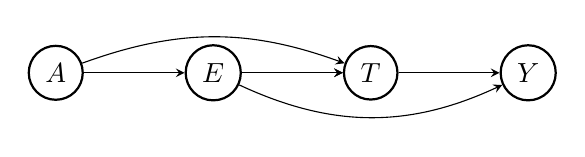
\begin{tikzpicture}
            [>=stealth, rv/.style={circle, draw, thick, minimum size=6mm}, rvc/.style={triangle, draw, thick, minimum size=10mm}, node distance=18mm]
            \pgfsetarrows{latex-latex};
            \begin{scope}
            \node[rv] (1) at (-2,0) {$A$};
            \node[rv] (2) at (0,0) {$E$};
            \node[rv] (3) at (2,0) {$T$};
            \node[rv] (4) at (4,0) {$Y$};
            \draw[->] (1) -- (2);
            \draw[->] (1) edge[bend left = 20] (3);
            \draw[->] (2) -- (3);
            \draw[->] (2) -- (3);
            \draw[->] (3) -- (4);
            \draw[->] (2) edge[bend right = 25] (4);
            \end{scope}
            \end{tikzpicture}
\end{center}

Attribute \(A\), gender, has a causal effect on variables \(E\), \(T\)
and \(Y\), and we wish to eliminate this effect. For each individual
with observed values \((a, e, t, y)\) we want to find a mapping
\[(a, e, t, y) \longrightarrow  ( {a}^{(fp)},  {e}^{(fp)},  {t}^{(fp)},  {y}^{(fp)}),\]
which finds the value the person would have obtained in a world where
everyone is female. Explicitly, for a male person with education value
\(e\), we give it the transformed value \( {e}^{(fp)}\) chosen such that
\[\mathbbm{P}(E \geq e \mid A = a') = \mathbbm{P}(E \geq  {e}^{(fp)} \mid A = a). \]
The main idea is that the
\textit{relative educational achievement within the subgroup} would stay
the same if we changed someone's gender. If you are male and you have a
higher educational achievement than 60\% of all males in the dataset, we
assume you would be better than 60\% of females had you been
female\footnote{This assumption is empirically untestable, since it is impossible to observe both a female and a male version of the same individual.}.
After computing everyone's education (in the `female' world), we
continue by computing the transformed test score values \( {T}^{(fp)}\).
The approach is again similar, but this time we condition on educational
achievement. That is, a male with values \((E, T) = (e, t)\) is assigned
a test score \( {t}^{(fp)}\) such that
\[\mathbbm{P}(T \geq t \mid E = e, A = a') = \mathbbm{P}(T \geq  {t}^{(fp)} \mid E =  {e}^{(fp)}, A = a),\]
where the value \( {e}^{(fp)}\) was obtained in the previous step. The
step can be visualized as
follows\footnote{In the visualization, the test scores of male applicants have higher values. We emphasize this is in no way a view implied by the authors, simply a currently observed societal bias in certain university admission datasets.}

\begin{center}
  \begin{tikzpicture}
    \begin{axis}[
    no markers, domain=0:10, samples=100,
    axis lines*=left, xlabel=$v$, ylabel=density,
    every axis y label/.style={at=(current axis.above origin),anchor=south},
    every axis x label/.style={at=(current axis.right of origin),anchor=west},
    height=5cm, width=12cm,
    xtick=\empty, ytick=\empty,
    enlargelimits=false, clip=false, axis on top,
    grid = major
    ]
  \addplot [very thick,green!50!black] {gauss(4,1)};
  \addplot [very thick,blue!50!black] {gauss(6.5,0.8)};
  \draw[-{Latex[length=3mm,width=2mm]}, dashed] (axis cs:5.474,0.219) to[bend left = 30] (axis cs:2.718,0.175);
  \draw[-{Latex[length=3mm,width=2mm]}, dashed] (axis cs:6.919520, 0.4346158) to[bend left = 30] (axis cs:4.524401, 0.3476926);

  \node at (axis cs:2.718,0.175) [above, left] {$10\%$ female};
  \node at (axis cs:5.474,0.219) [right] {$10\%$ male};
  \node at (axis cs:4.524401, 0.3476926) [above=0.5cm] {$70\%$ female};
  \node at (axis cs:6.919520, 0.4346158) [right] {$70\%$ male};

  \node at (axis cs:4,0.5) [below = 0.65cm, left = 0.4cm, green!50!black] {$T \mid E = e, A = a'$};
  \node at (axis cs:6.5,0.5) [below = 1cm, right = 0.9cm, blue!50!black] {$T \mid E =  {e}^{(fp)}, A = a$};

  \end{axis}

  \end{tikzpicture}
\end{center}

In the last step, the outcome variable \(Y\) needs to be adjusted. The
adaptation is based on the values of education and the test score. The
transformed value \( {y}^{(fp)}\) of \(Y = y\) would satisfy
\begin{equation} \label{eq:labeltransform}
    \mathbbm{P}(Y \geq y \mid E = e, T = t, A = a') = \mathbbm{P}(Y \geq  {y}^{(fp)} \mid E =  {e}^{(fp)}, T =  {t}^{(fp)}, A = a).
\end{equation} This way of counterfactual correction is known as
\textit{recursive substitution} \citep[Chapter~7]{pearl2009}.

We next describe the approach from above formally. The reader who is not
interested in the mathematical detail is encouraged to go straight to
Section \ref{Implementation}. We start by introducing an important
causal inference concept, related to our discussion, namely the
\textit{structural causal model}. A structural causal model (SCM) is a
4-tuple \(<V, U, \mathcal{F}, P(u)>\), where

\begin{itemize}
    \item $V = \lbrace V_1, ..., V_n \rbrace$ is the set of observed (endogeneous) variables
    \item $U = \lbrace U_1, ..., U_n \rbrace$ are latent (exogeneous) variables
    \item $\mathcal{F} = \lbrace f_1, ..., f_n \rbrace$ is the set of functions determining $V$, $v_i \gets f_i(\mathrm{pa}(v_i), u_i)$, where $\mathrm{pa}(V_i) \subset V, U_i \subset U$ are the functional arguments of $f_i$
    \item $P(u)$ is a distribution over the exogeneous variables $U$.
  \end{itemize}

We note that any particular SCM is accompanied by a graphical model
\(\mathcal{G}\) (a directed acyclic graph), which summarizes which
functional arguments are necessary for computing the values of each
\(V_i\) (that it is, how variables affect each other). We assume
throughout, without loss of generality, that

\begin{enumerate}[(i)]
            \item $f_i(\mathrm{pa}(v_i), u_i)$ is increasing in $u_i$ for every fixed $\mathrm{pa}(v_i)$
            \item exogeneous variables $U_i$ are uniformly distributed on $[0, 1]$
\end{enumerate}

We first discuss the so-called Markovian case in which all exogeneous
variables \(U_i\) are mutually independent. Some relevant extensions,
like the Semi-Markovian case (where \(U_i\) variables are allowed to
have mutual dependencies) and the case of so called
\textit{resolving variables}, are discussed in Section \ref{Extensions}.

\hypertarget{basic-formulation---markovian-scms}{%
\subsection{Basic formulation - Markovian
SCMs}\label{basic-formulation---markovian-scms}}

Suppose that \(Y\) taking values in \(\mathbbm{R}\) is an outcome of
interest and \(A\) the protected attribute taking two values \(a, a'\).
Our goal is to describe a pre-processing method which transform the
entire data \(V\) into its fair version \( {V}^{(fp)}\). This is done by
computing the counterfactual values \(V(A = a)\) which would have been
obtained by the individuals, had everyone had the same protected
attribute \(A = a\).

More precisely, going back to the \emph{university admission} example
above, we want to ``equate'' the distributions \begin{equation}
  V_i \mid \mathrm{pa}(V_i), A = a \text{ and } V_i \mid \mathrm{pa}(V_i), A = a'.
\end{equation} In words, we want the distribution of \(V_i\) to be the
same for the female and male applicants, for every variable \(V_i\).
Since each function \(f_i\) of the original SCM is reparametrized so
that \(f_i(\mathrm{pa}(v_i), u_i)\) is increasing in \(u_i\) for every
fixed \(\mathrm{pa}(v_i)\), and also that \(U_i\) variables are
uniformly distributed on \([0, 1]\). Then the \(U_i\) variables can be
seen as the latent \textit{quantiles}. Our algorithm proceedes as
follows:

\begin{algorithm}
    \DontPrintSemicolon
    \KwIn{$V$, causal graph $\mathcal{G}$}
    set $A \gets a$ for everyone\\
    \For{$V_i \in \mathrm{de}(A)$ in topological order}{
      learn the assignment function $V_i \gets f_i(\mathrm{pa}(V_i), U_i)$ \;
        infer the quantiles $U_i$ associated with the variable $V_i$\;
        transform the values of $V_i$ by using the quantile and the transformed parents (obtained in previous steps)
        $ {V_i}^{(fp)} \gets f_i ( {\mathrm{pa}(V_i)}^{(fp)}, U_i)$ \;
  }
  \Return{$ {V}^{(fp)}$}
    \caption{{\sc Fair Data Adaptation}}
    \label{algo:fairadapt}
\end{algorithm}

The \(f_i\) assignment functions of the SCM are of course unknown, but
are learned non-parametrically at each step. Notice that Algorithm
\ref{algo:fairadapt} is computing the counterfactual values \(V(A = a)\)
under the \(do(A = a)\) intervention for each individual, while keeping
the latent quantiles \(U\) fixed. In the case of continuous variables,
the latent quantiles \(U\) can be determined exactly, while for the
discrete case, this is more subtle and described in detail in the
original fair data adaptation manuscript
\citep[Section~5]{plecko2020fair}.

\hypertarget{implementation}{%
\section{Implementation}\label{implementation}}

\label{Implementation}

The implementation is based on the main function \texttt{fairadapt()},
which returns an S3 object of class \texttt{"fairadapt"}. We list the
most important arguments of the function and then show how these should
be specified:

\begin{itemize}
\tightlist
\item
  \texttt{formula}, argument of type \texttt{formula} specifies the
  dependent and explanatory variables
\item
  \texttt{adj.mat} argument of type \texttt{matrix} encodes the
  adjacency matrix
\item
  \texttt{train.data}, \texttt{test.data} of type \texttt{data.frame}
\item
  \texttt{protect.A} of type \texttt{character} is of length one and
  names the protected attribute.
\end{itemize}

\begin{CodeChunk}
\begin{CodeInput}
R> uni.adj.mat <- array(0, dim = c(4, 4))
R> colnames(uni.adj.mat) <- rownames(uni.adj.mat) <-
+   c("gender", "edu", "test", "score")
R> 
R> uni.adj.mat["gender", c("edu", "test")] <-
+   uni.adj.mat["edu", c("test", "score")] <-
+   uni.adj.mat["test", "score"] <- 1L
R> 
R> nsamp <- 200
R> 
R> FA.basic <- fairadapt(score ~ .,
+   train.data = uni_admission[1:nsamp, ],
+   test.data = uni_admission[(nsamp+1):(2*nsamp), ],
+   adj.mat = uni.adj.mat, protect.A = "gender", res.vars = NULL,
+   visualize.graph = F, quant.method = fairadapt:::rangerQuants)
R> 
R> FA.basic
\end{CodeInput}
\begin{CodeOutput}
Fairadapt result

Call:
 score ~ . 

Protected attribute:                  gender 
Protected attribute levels:           0, 1 
Number of training samples:           200 
Number of test samples:               200 
Number of independent variables:      3 
Total variation (before adaptation):  -0.6757414 
Total variation (after adaptation):   -0.1014389 
\end{CodeOutput}
\end{CodeChunk}

The \texttt{"fairadapt"} \texttt{S3} class has several associated
generics and methods. For instance, \texttt{print(FA.basic)} shows some
information about the object call, such as number of variables, the
protected attribute and also the total variation before and after
adaptation, defined as (\(Y\) denoting the outcome variable)
\[\mathbbm{E}[Y \mid A = a] - \mathbbm{E}[Y \mid A = a'] \text{ and } \mathbbm{E}[ {Y}^{(fp)} \mid A = a] - \mathbbm{E}[ {Y}^{(fp)} \mid A = a'],\]
respectively. The total variation, in the case of binary \(Y\),
corresponds to the parity gap.

\hypertarget{specifying-the-graphical-model}{%
\subsection{Specifying the graphical
model}\label{specifying-the-graphical-model}}

The \pkg{fairadapt} supposes the underlying graphical model
\(\mathcal{G}\) is known. The model is specified by the adjacency
matrix. For example, suppose we take the causal graph \(\mathcal{G}\) of
the university admission example above. For such a graph, we construct
the adjacency matrix and the graph with the \texttt{GraphModel()}
convenience function that builds on top of the \pkg{igraph} package.

\begin{CodeChunk}
\begin{CodeInput}
R> toy.graph <- graphModel(uni.adj.mat)
R> plot(toy.graph, vertex.size = 40, vertex.label.cex = 0.5,
+   vertex.label.color = "black")
\end{CodeInput}


\begin{center}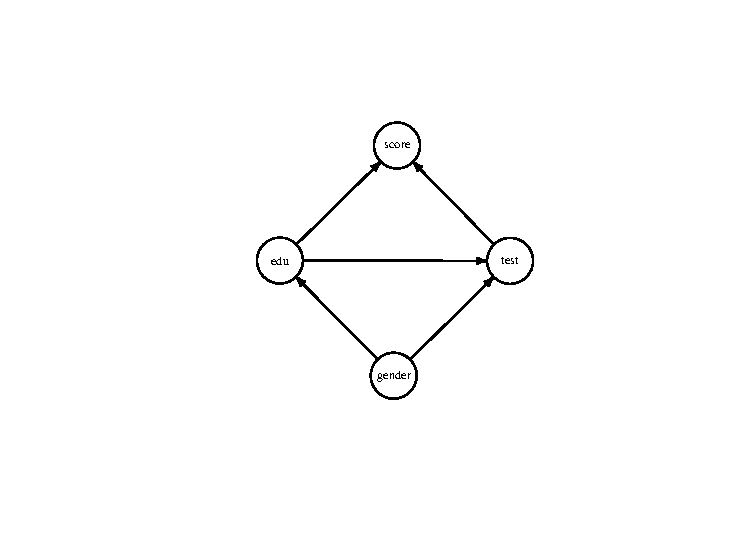
\includegraphics[width=200px,height=200px]{/private/var/folders/24/8k48jl6d249_n_qfxwsl6xvm0000gn/T/RtmpOjXPo8/file7af3350ee0/dev/articles/jss_files/figure-latex/mat-1} \end{center}

\end{CodeChunk}

\hypertarget{quantile-learning-step}{%
\subsection{Quantile learning step}\label{quantile-learning-step}}

We describe the training step using the \texttt{fairadapt()} function.
The \texttt{fairadapt()} function can be used in two slightly distinct
ways. The first option is by specifying training and testing data at the
same time. The data adaptation is then applied to the combination of
train and test data, in order to learn the latent quantiles as precisely
as possible (with the exception of label \(Y\) which is unavailable on
the test set). The second option is use only the \texttt{train.data}
argument when calling \texttt{fairadapt()}, after which the
\texttt{predict()} function can be used to adapt test data at a later
stage.

We note that \texttt{train.data} and \texttt{test.data} need to have
column names which appear in the names of the adjacency matrix
\texttt{colnames(adj.mat)}. The protected attribute \(A\) is given as a
character vector \texttt{protect.A} of length one.

The quantile learning step in Algorithm \ref{algo:fairadapt} can be done
using three different methods:

\begin{itemize}
\item Quantile Regression Forests \citep{qrf}
\item Non-crossing quantile neural networks \citep{cannon2018non}
\item Linear Quantile Regression \citep{qr}
\end{itemize}

The summary of the various differences between the methods is given in
Table \ref{tab:qmethods}.

\begin{table}
    \centering
    \begin{tabular}{>{\centering\arraybackslash} m{3.5cm}| >{\centering\arraybackslash} m{3cm} >{\centering\arraybackslash}m{3cm} >{\centering\arraybackslash}m{3cm}}
  & Random Forests & Neural Networks & Linear Regression \\ \hline
  \texttt{R}-package & \pkg{ranger} & \pkg{mcqrnn} & \pkg{quantreg} \\ \hline
  \texttt{quant.method} & \code{rangerQuants} & \code{mcqrnnQuants} & \code{linearQuants} \\ \hline
  complexity & $O(np\log n)$ & $O(npn_{\text{epochs}})$ & $O(p^2n)$ \\ \hline
  default parameters & $ntrees = 500$ \newline $mtry = \sqrt{p}$ & 2-layer fully connected feed-forward network & \code{"br"} method of Barrodale and Roberts used for fitting \\ \hline
  $T(200, 4)$ & $0.4$ sec & $89$ sec & $0.3$ sec \\ \hline
  $T(500, 4)$ & $0.9$ sec & $202$ sec & $0.5$ sec \\ \hline
\end{tabular}
    \caption{Summary table of different quantile regression methods. $n$ is the number of samples, $p$ number of covariates, $n_{\text{epochs}}$ number of training epochs for the NN. $T(n, 4)$ denotes the runtime of different methods on the university admission dataset, with $n$ training and testing samples.}
    \label{tab:qmethods}
\end{table}

The choice of quantile learning method is done by specifying the
\texttt{quant.method} argument, which is of class \texttt{function} and
constructs the quantile regression object. For more details and an
example, see \texttt{?rangerQuants}. Together with the
\texttt{quant.method} constructor, \texttt{S3}-dispatch is used for
inferring the quantiles. This allows the user to specify their own
quantile learning methods easily.

We quickly discuss the quantile learning methods included in the
package. Using the linear quantile method is the fastest option.
However, it cannot handle the non-parametric case. For a non-parametric
approach and mixed data, the RF approach is well-suited. The neural
network approach is, comparatively, substantially slower than the
forest/linear case and does not scale well to large sample sizes.
Generally, we recommend using the forest based approach, because of the
non-parametric nature and computational speed. However, we note that for
smaller sample sizes, the neural network approach might in fact be the
best option.

\hypertarget{fair-twin-inspection}{%
\subsection{Fair-twin inspection}\label{fair-twin-inspection}}

The university admission example presented in Section \ref{Method}
demonstrates how we can compute counterfactual values for an individual
while preserving their relative educational achievement. In particular,
for a male student with values \((a, e, t, y)\), we compute his
``fair-twin'' values
\(( {a}^{(fp)},  {e}^{(fp)},  {t}^{(fp)},  {y}^{(fp)})\) - the values
the student would have obtained, had he been female. To explicitly
compare a person to their hypothetical fair-twin, we use the
\texttt{fairTwins()} function, applied to an object of class
\texttt{"fairadapt"}:

\begin{CodeChunk}
\begin{CodeInput}
R> fairTwins(FA.basic, train.id = seq.int(1L, 5L, 1L))
\end{CodeInput}
\begin{CodeOutput}
  gender      score score_adapted        edu edu_adapted         test
1      1  1.9501728    1.22758002  1.3499572  0.51083985  1.617739679
2      0 -2.3502495   -2.35024955 -1.9779234 -1.97792341 -3.121796235
3      1  0.6285619   -0.04234933  0.6263626 -0.05711465  0.530034686
4      1  0.7064857    0.13173095  0.8142112  0.18782225  0.004573003
5      1  0.3678313    0.23076887  1.8415242  0.93119184  1.193677123
  test_adapted
1    0.6413782
2   -3.1217962
3   -0.5822567
4   -0.7734410
5    0.5390240
\end{CodeOutput}
\end{CodeChunk}

In this example, we compute the values in a ``female'' world. Therefore,
for female applicants, the values stay the same, while for male
applicants the values are adapted, as can be seen from the output.

\hypertarget{illustration}{%
\section{Illustration}\label{illustration}}

\label{Illustration} Here we describe an example of a possible
real-world use of \pkg{fairadapt}. Suppose that after a legislative
change the US government has decided to adjust the salary of all of its
female employees in order to remove both disparate treatment and
disparate impact effects. To this end, the government wants to compute
the counterfactual salary values of all female employees, that is the
salaries that female employees would obtain, had they been male.

To do this, the government is using the from the 2018 American Community
Survey by the US Census Bureau. We load the pre-processed version of the
dataset:

\begin{CodeChunk}
\begin{CodeInput}
R> dat <- gov_census
R> print(head(dat))
\end{CodeInput}
\begin{CodeOutput}
      sex age  race hispanic_origin citizenship nativity  marital family_size
1:   male  64 black              no           1   native  married           2
2: female  54 white              no           1   native  married           3
3:   male  38 black              no           1   native  married           3
4: female  41 asian              no           1   native  married           3
5: female  40 white              no           1   native  married           4
6: female  46 white              no           1   native divorced           3
   children education_level english_level salary hours_worked weeks_worked
1:        0              20             0  43000           56           49
2:        1              20             0  45000           42           49
3:        1              24             0  99000           50           49
4:        1              24             0  63000           50           49
5:        2              21             0  45200           40           49
6:        1              18             0  28000           40           49
   occupation industry economic_region
1:    13-1081     928P       Southeast
2:    29-2061     6231       Southeast
3:    25-1000    611M1       Southeast
4:    25-1000    611M1       Southeast
5:    27-1010    611M1       Southeast
6:    43-6014     6111       Southeast
\end{CodeOutput}
\begin{CodeInput}
R> # group the columns
R> protect.A <- "sex"
R> dmgraph <- c("age", "race", "hispanic_origin", "citizenship", "nativity",
+   "economic_region")
R> fam <- c("marital", "family_size", "children")
R> edu <- c("education_level", "english_level")
R> work <- c("hours_worked", "weeks_worked", "occupation", "industry")
R> out <- "salary"
\end{CodeInput}
\end{CodeChunk}

The hypothesized causal graph for the dataset is given in Figure
\ref{fig:censusgraph}. We construct the causal graph and the confounding
matrix:

\begin{CodeChunk}
\begin{CodeInput}
R> col.names <- c(protect.A, dmgraph, fam, edu, work, out)
R> 
R> adj.mat <- cfd.mat <- array(0, dim = c(length(col.names), length(col.names)))
R> colnames(adj.mat) <- rownames(adj.mat) <-
+   colnames(cfd.mat) <- rownames(cfd.mat) <-
+   col.names
R> 
R> adj.mat[protect.A, c(fam, edu, work, out)] <-
+   adj.mat[dmgraph, c(fam, edu, work, out)] <-
+   adj.mat[fam, c(edu, work, out)] <-
+   adj.mat[edu, c(work, out)] <-
+   adj.mat[work, out] <-
+   cfd.mat[protect.A, dmgraph] <- cfd.mat[dmgraph, protect.A] <- 1L
R> 
R> census.graph <- graphModel(adj.mat, cfd.mat)
R> plot(census.graph, vertex.size = 20, vertex.label.cex = 0.5,
+   vertex.label.color = "black")
\end{CodeInput}


\begin{center}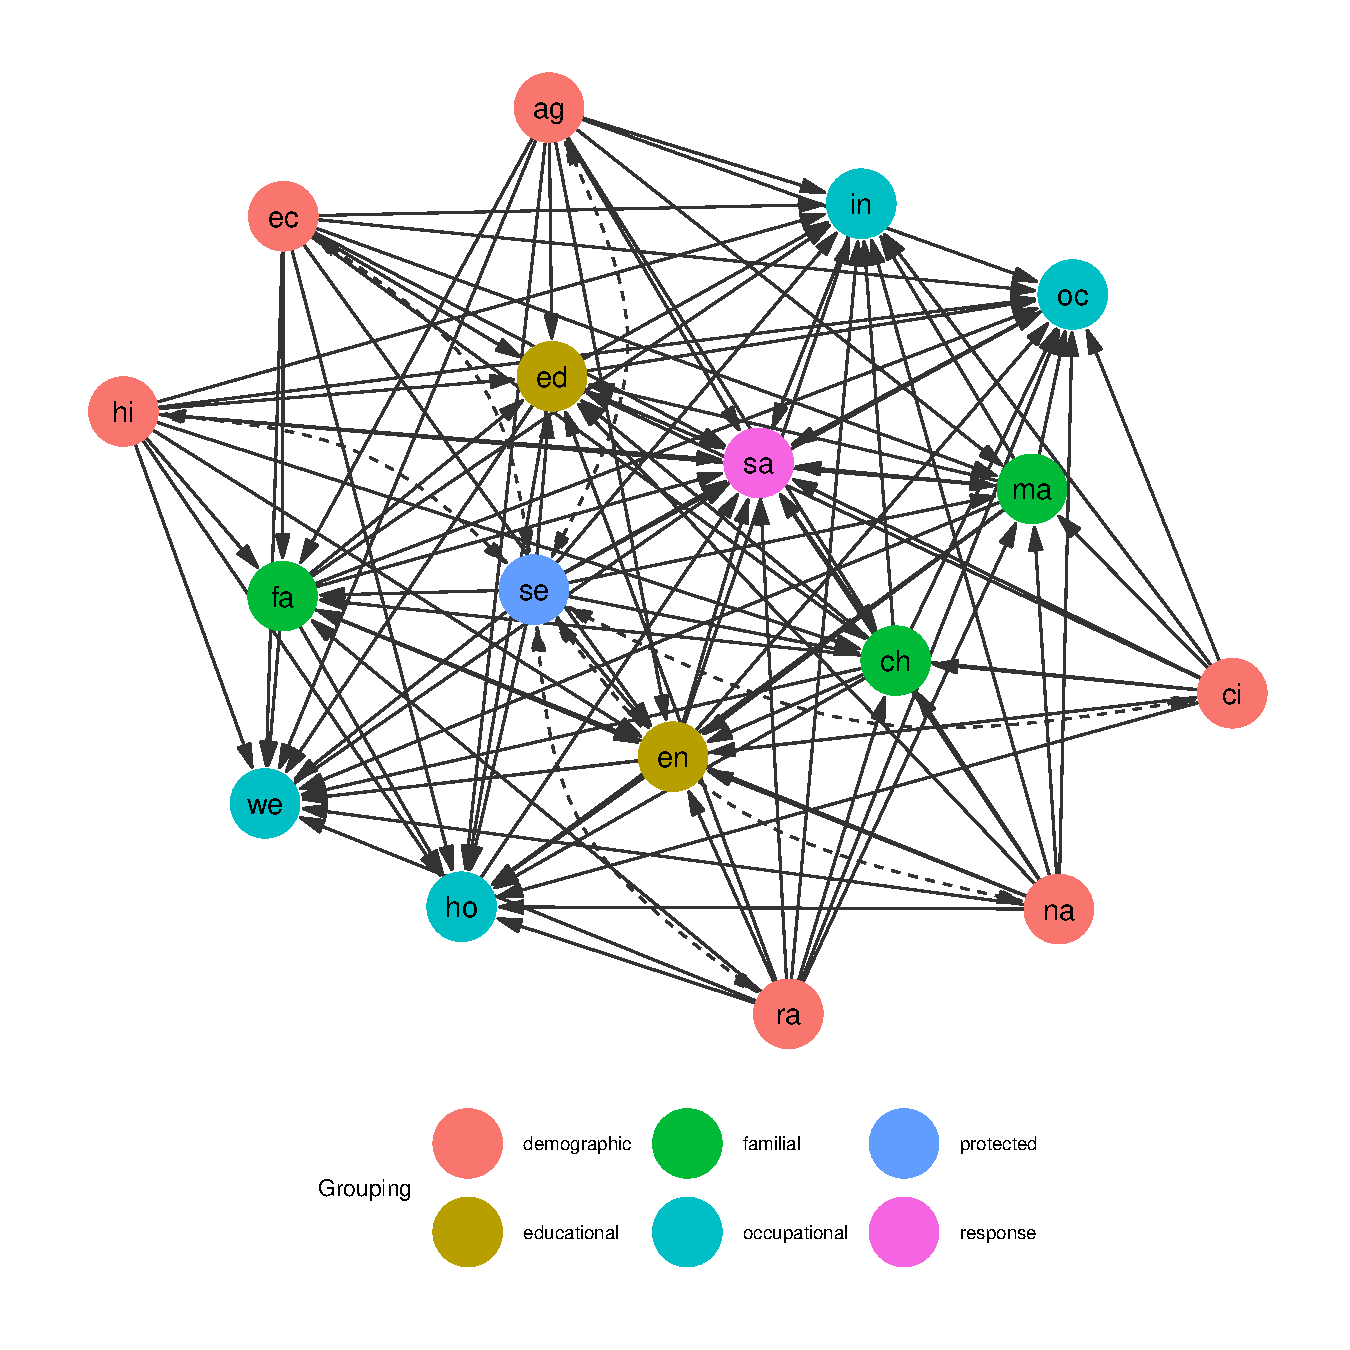
\includegraphics{/private/var/folders/24/8k48jl6d249_n_qfxwsl6xvm0000gn/T/RtmpOjXPo8/file7af3350ee0/dev/articles/jss_files/figure-latex/census-graph-1} \end{center}

\end{CodeChunk}

\begin{figure} \centering
    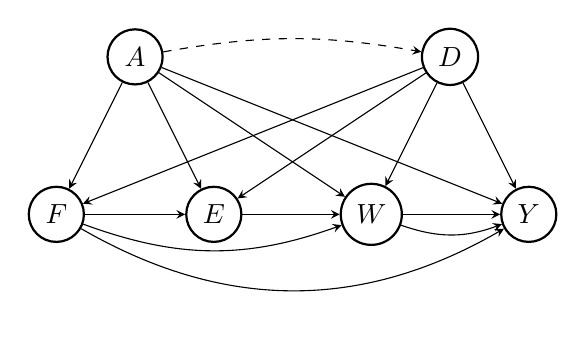
\begin{tikzpicture}
    [>=stealth, rv/.style={circle, draw, thick, minimum size=7mm}, rvc/.style={triangle, draw, thick, minimum size=8mm}, node distance=7mm]
    \pgfsetarrows{latex-latex};
    \begin{scope}
    \node[rv] (c) at (2,2) {$D$};
    \node[rv] (a) at (-2,2) {$A$};
    \node[rv] (m) at (-3,0) {$F$};
    \node[rv] (l) at (-1,0) {$E$};
    \node[rv] (r) at (1,0) {$W$};
    \node[rv] (y) at (3,0) {$Y$};
    \draw[->] (c) -- (m);
    \draw[->] (c) -- (l);
    \draw[->] (c) -- (r);
    \draw[->] (c) -- (y);
    \draw[->] (a) -- (m);
    \draw[->] (m) -- (l);
    \draw[->] (l) -- (r);
    \draw[->] (r) -- (y);
    \path[->] (a) edge[bend left = 0] (l);
    \path[->] (a) edge[bend left = 0] (r);
    \path[->] (a) edge[bend left = 0] (y);
    \path[->] (m) edge[bend right = 20] (r);
    \path[->] (m) edge[bend right = 30] (y);
    \path[->] (r) edge[bend right = 20] (y);
    \path[->, dashed] (a) edge[bend left = 10] (c);
    \end{scope}
    \end{tikzpicture}
    \caption{The causal graph for the Government-Census dataset. $D$ are demographic features, $A$ is gender, $F$ is marital and family information, $E$ education, $W$ work-related information, $Y$ the salary, which is also the outcome of interest.}
    \label{fig:censusgraph}
\end{figure}

Before applying \texttt{fairadapt()}, we first log-transform the
salaries and look at the densities by gender group

\begin{CodeChunk}
\begin{CodeInput}
R> # log-transform the salaries
R> dat$salary <- log(dat$salary)
R> 
R> # plot density before adaptation
R> nsamples <- 2000
R> 
R> ggplot(dat[1:nsamples], aes(x = salary, fill = sex)) +
+   geom_density(alpha = 0.4)  + theme_minimal() +
+   ggtitle("Salary density by gender")
\end{CodeInput}


\begin{center}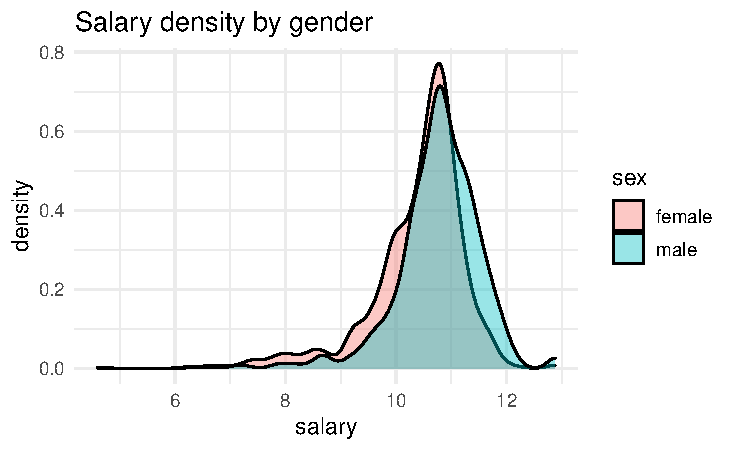
\includegraphics{/private/var/folders/24/8k48jl6d249_n_qfxwsl6xvm0000gn/T/RtmpOjXPo8/file7af3350ee0/dev/articles/jss_files/figure-latex/log-and-graph-1} \end{center}

\end{CodeChunk}

There is a clear shift between the two genders, meaning that
\texttt{male} employees are currently treated better than
\texttt{female} employees. However, there could be differences in
\texttt{salary} which are not due to gender inequality, but have to do
with the economic region in which the employee works. This needs to be
accounted for as well, i.e.~the difference between economic regions is
not to be removed. To solve the problem, the US governemnt applies
\pkg{fairadapt}:

\begin{CodeChunk}
\begin{CodeInput}
R> FA.govcensus <- fairadapt(salary ~ ., train.data = dat[1:nsamples],
+                           adj.mat = adj.mat, protect.A = protect.A,
+                           visualize.graph = F)
\end{CodeInput}
\end{CodeChunk}

After applying the adaptation, we inspect whether the problem has
improved. The densities after adaptation can be plotted using the
\texttt{autoplot()} function:

\begin{CodeChunk}
\begin{CodeInput}
R> autoplot(FA.govcensus, when = "after") +
+   ggtitle("Adapted salary density by gender")
\end{CodeInput}


\begin{center}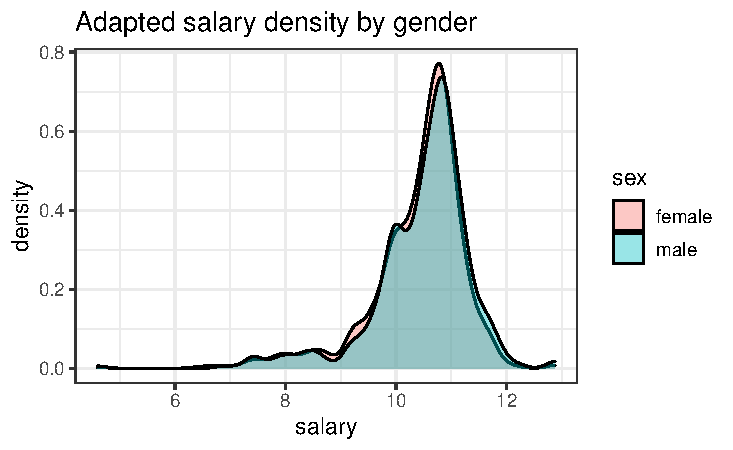
\includegraphics{/private/var/folders/24/8k48jl6d249_n_qfxwsl6xvm0000gn/T/RtmpOjXPo8/file7af3350ee0/dev/articles/jss_files/figure-latex/vis-adapt-1} \end{center}

\end{CodeChunk}

If we obtain additional testing data, and wish to adapt it as well, we
can use the \texttt{predict()} function:

\begin{CodeChunk}
\begin{CodeInput}
R> new.test <- dat[seq.int(nsamples + 1L, nsamples + 10L, 1L)]
R> adapt.test <- predict(FA.govcensus, newdata = new.test)
R> head(adapt.test)
\end{CodeInput}
\begin{CodeOutput}
      sex age  race hispanic_origin citizenship nativity marital family_size
1: female  52 white              no           1   native married           3
2: female  31 white              no           1   native married           5
3: female  53 white              no           1   native married           2
4: female  53 black              no           1   native married           2
5: female  23 white              no           1   native married           2
6: female  49 white             yes           1   native married           7
   children education_level english_level   salary hours_worked weeks_worked
1:        1              21             0 11.91839        40.00           49
2:        3              22             0 10.77896        40.00           49
3:        0              22             0 11.40756        40.00           49
4:        0              21             0 11.28978        40.00           49
5:        0              22             0 10.46310        19.94           49
6:        4              22             0 10.69194        40.00           49
   occupation industry economic_region
1:    13-1082     92M2       Southeast
2:    25-2020     6111       Southeast
3:    25-1000    3132Z       Southeast
4:    11-91XX     928P       Southeast
5:    43-9XXX     6216       Southeast
6:    25-2020     6111       Southeast
\end{CodeOutput}
\end{CodeChunk}

Finally, we can do fair-twin inspection using the \texttt{fairTwins()}
function, to see how feature values of individual employees have
changed:

\begin{CodeChunk}
\begin{CodeInput}
R> inspect.cols <- c("sex", "age", "education_level", "salary")
R> fairTwins(FA.govcensus, train.id = 1:5, cols = inspect.cols)
\end{CodeInput}
\begin{CodeOutput}
     sex age age_adapted education_level education_level_adapted   salary
1   male  64          64              20                      19 10.66896
2 female  54          54              20                      20 10.71442
3   male  38          38              24                      24 11.50288
4 female  41          41              24                      24 11.05089
5 female  40          40              21                      21 10.71885
  salary_adapted
1       9.903488
2      10.714418
3      11.643954
4      11.050890
5      10.718852
\end{CodeOutput}
\end{CodeChunk}

The values are unchanged for the female individuals. Note that
\texttt{age} does not change for any individual, since it is not a
descendant of \(A\). However, variables \texttt{education\_level} and
\texttt{salary} do change for males, as they are descendants of \(A\).

The variable \texttt{hours\_worked} is also a descendant of \(A\).
However, one might argue that this variable should not be adapted in the
procedure, that is, that it should remain the same, even if we
hypothetically change the person's gender. This is the idea behind
\textit{resolving variables}, introduced in the next section.

\hypertarget{extensions}{%
\section{Extensions}\label{extensions}}

\label{Extensions}

\hypertarget{adding-resolving-variables}{%
\subsection{Adding resolving
variables}\label{adding-resolving-variables}}

\cite{kilbertus2017avoiding} discuss that in some situations the
protected attribute \(A\) can affect variables in a non-discriminatory
way. For instance, in the Berkeley admissions dataset
\citep{bickel1975sex} we observe that females often apply for
departments with lower admission rates and consequently have a lower
admission probability. However, we perhaps would not wish to account for
this difference in the adaptation procedure if we were to argue that
department choice is a choice everybody is free to make. This motivated
the following reasoning, found in \citet{kilbertus2017avoiding}. A
variable \(R\) is called resolving if

\begin{enumerate}[(i)]
        \item $R \in \mathrm{de}(A)$, where $\mathrm{de}(A)$ are the descendants of $A$ in the causal graph $\mathcal{G}$
        \item the causal effect of $A$ on $R$ is considered to be non-discriminatory
\end{enumerate}

In presence of resolving variables, we compute the counterfactual under
a more complicated intervention do\((A = a, R = R(a'))\). The potential
outcome value \(V(A = a, R = R(a'))\) is obtained by setting \(A = a\)
and computing the counterfactual while keeping the values of resolving
variables to those they \textit{attained naturally}. This is a nested
counterfactual and the difference in Algorithm \ref{algo:fairadapt} is
simply that resolving variables \(R\) are skipped over in the for-loop.
We run the following code to compute the fair adaptation with the
variable \texttt{test} being resolving in the \texttt{uni\_admission}
dataset

\begin{CodeChunk}
\begin{CodeInput}
R> FA.resolving <- fairadapt(score ~ .,
+   train.data = uni_admission[1:nsamp, ],
+   test.data = uni_admission[(nsamp+1):(2*nsamp), ],
+   adj.mat = uni.adj.mat, protect.A = "gender", res.vars = "test",
+   visualize.graph = F)
R> 
R> FA.resolving
\end{CodeInput}
\begin{CodeOutput}
Fairadapt result

Call:
 score ~ . 

Protected attribute:                  gender 
Protected attribute levels:           0, 1 
Resolving variables:                  test 
Number of training samples:           200 
Number of test samples:               200 
Number of independent variables:      3 
Total variation (before adaptation):  -0.6757414 
Total variation (after adaptation):   -0.4268619 
\end{CodeOutput}
\end{CodeChunk}

We note that the total variation in this case is larger than in the
\texttt{FA.basic} example from Section \ref{Implementation}, with no
resolvers. The intuitive reasoning here is that resolving variables
allow for some discrimination, so we expect to see a larger total
variation between the groups. Finally, we can visualize the graph

\begin{CodeChunk}
\begin{CodeInput}
R> plot(graphModel(uni.adj.mat, res.vars = "test"),
+   vertex.size = 40, vertex.label.cex = 0.5,
+   vertex.label.color = "black")
\end{CodeInput}


\begin{center}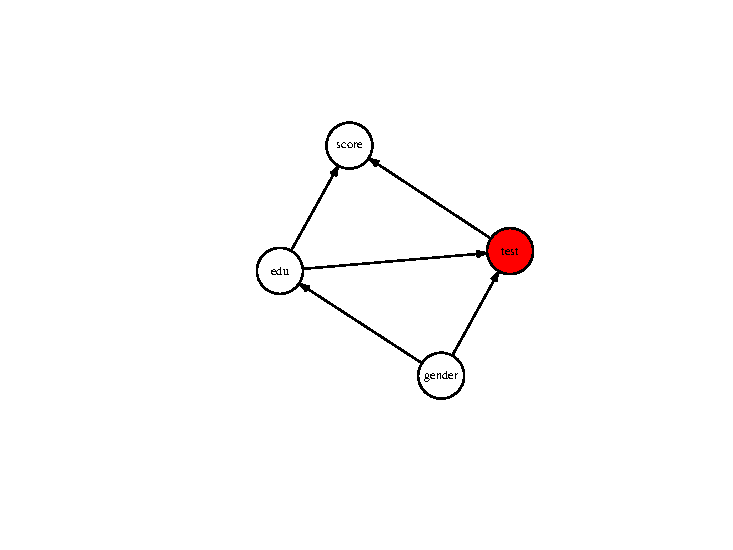
\includegraphics[width=200px,height=200px]{/private/var/folders/24/8k48jl6d249_n_qfxwsl6xvm0000gn/T/RtmpOjXPo8/file7af3350ee0/dev/articles/jss_files/figure-latex/resolving-graph-1} \end{center}

\end{CodeChunk}

which shows a different color for the resolving variable \texttt{test}.
The resolving variables are red-colored in order to be distinguished
from other variables.

\hypertarget{semi-markovian-and-topological-ordering-variant}{%
\subsection{Semi-Markovian and topological ordering
variant}\label{semi-markovian-and-topological-ordering-variant}}

In Section \ref{Method} we were concerned with the Markovian case, which
assumes that all exogeneous variables \(U_i\) are mutually independent.
However, in practice this need not be the case. If there are mutual
dependencies between the \(U_i\)s, we are dealing with a so-called
Semi-Markovian model. These dependencies between latent variables are
represented by dashed, bidirected arrows in the causal diagram. In the
university admission example, suppose we had that
\(U_{\text{test}} \not\!\perp\!\!\!\perp U_{\text{score}}\), meaning
that latent variables corresponding to variable test and final score are
correlated. Then the graphical model would be represented as

\begin{center}
    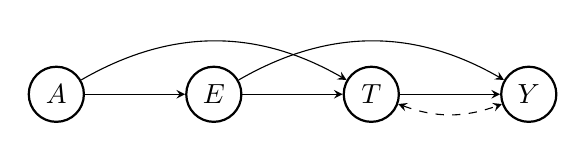
\begin{tikzpicture}
    [>=stealth, rv/.style={circle, draw, thick, minimum size=7mm}, rvc/.style={triangle, draw, thick, minimum size=8mm}, node distance=7mm]
    \pgfsetarrows{latex-latex};
    \begin{scope}
    \node[rv] (a) at (-3,0) {$A$};
    \node[rv] (v1) at (-1,0) {$E$};
    \node[rv] (v2) at (1,0) {$T$};
    \node[rv] (y) at (3,0) {$Y$};
    \draw[->] (a) -- (v1);
    \draw[->] (a) edge[bend left = 30] (v2);
    \draw[->] (v1) -- (v2);
    \draw[->] (v1) edge[bend left = 30] (y);
    \draw[->] (v2) -- (y);
    \path[<->, dashed] (v2) edge[bend right = 20] (y);
    \end{scope}
    \end{tikzpicture}
\end{center}

There is an important difference in the adaptation procedure for
Semi-Markovian case: when inferring the latent quantiles \(U_i\) of
variable \(V_i\), in the Markovian case, only the direct parents
\(\mathrm{pa}(V_i)\) are needed. In the Semi-Markovian case, due to
correlation of latent variables, using only the \(\mathrm{pa}(V_i)\) can
lead to biased estimates of the \(U_i\). Instead, the set of direct
parents needs to be extended, described in detail in
\citep{tian2002general}. We briefly sketch the argument. Let the
\textit{C-components} be a partition of the set \(V\), such that each
\(C-component\) contains a set of variables which are mutually connect
by bidirected arrows. Let \(C(V_i)\) denote the whole C-component of
variable \(V_i\). We then define the set of extended parents
\[\mathrm{Pa}(V_i) := (C(V_i) \cup pa(C(V_i))) \cap \mathrm{an}(V_i),\]
where \(\mathrm{an}(V_i)\) are the ancestors of \(V_i\). The adaptation
procedure in the Semi-Markovian case remains the same as in Algorithm
\ref{algo:fairadapt}, with the difference that the set of direct parents
\(\mathrm{pa}(V_i)\) is replaced by \(\mathrm{Pa}(V_i)\) at each step.

To include the bidirected confounding arcs in the adaptation, we use the
\texttt{cfd.mat} argument of type \texttt{matrix} such that

\begin{itemize}
\tightlist
\item
  \texttt{cfd.mat} has the same dimension, column and row names as
  \texttt{adj.mat}
\item
  \texttt{cfd.mat} is symmetric and setting
  \texttt{cfd.mat{[}"Vi",\ "Vj"{]}\ \textless{}-\ cfd.mat{[}"Vj",\ "Vi"{]}\ \textless{}-\ 1L}
  indicates that there is a bidirected edge between variables \(V_i\)
  and \(V_j\).
\end{itemize}

Alternatively, instead of using the extended parent set
\(\mathrm{Pa}(V_i)\), we can use the ``largest possible'' set of
parents, namely the ancestors \(\mathrm{an}(V_i)\). This approach is
implemented, and the user only needs to specify the topological
ordering. This is done by specifying the \texttt{top.ord} argument which
is a \texttt{character} vector, containing the correct ordering of the
names appearing in \texttt{names(train.data)}.

The following code runs the adaptation in the Semi-Markovian case:

\begin{CodeChunk}
\begin{CodeInput}
R> uni.cfd.mat <- array(0, dim = c(4, 4))
R> colnames(uni.cfd.mat) <- rownames(uni.cfd.mat) <- colnames(uni.adj.mat)
R> 
R> uni.cfd.mat["test", "score"] <- uni.cfd.mat["score", "test"] <- 1L
R> FA.semimarkov <- fairadapt(score ~ .,
+   train.data = uni_admission[1:nsamp, ],
+   test.data = uni_admission[(nsamp+1):(2*nsamp), ],
+   adj.mat = uni.adj.mat, cfd.mat = uni.cfd.mat, protect.A = "gender",
+   visualize.graph = F)
\end{CodeInput}
\end{CodeChunk}

We visualize the graph that was used for the adaptation.

\begin{CodeChunk}
\begin{CodeInput}
R> plot(FA.semimarkov, graph = T, vertex.size = 40,
+   vertex.label.cex = 0.5, vertex.label.color = "black")
\end{CodeInput}


\begin{center}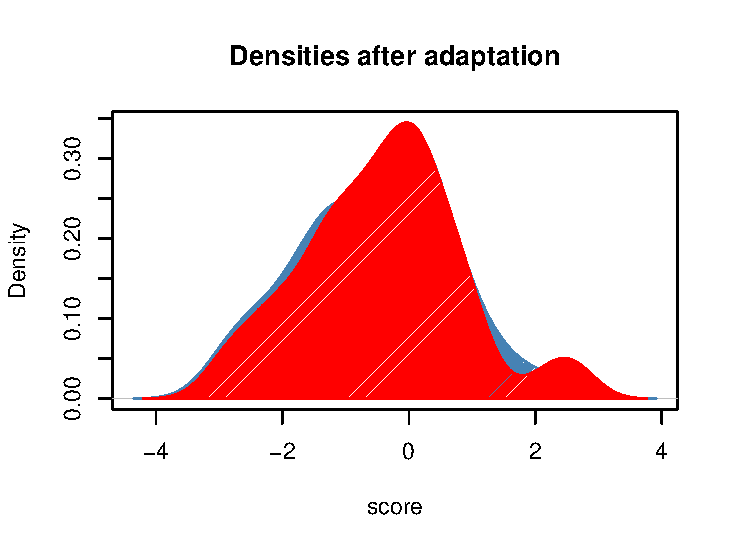
\includegraphics[width=200px,height=200px]{/private/var/folders/24/8k48jl6d249_n_qfxwsl6xvm0000gn/T/RtmpOjXPo8/file7af3350ee0/dev/articles/jss_files/figure-latex/graph-semimarkov-1} \end{center}

\end{CodeChunk}

\hypertarget{questions-of-identifiability}{%
\subsection{Questions of
identifiability}\label{questions-of-identifiability}}

So far, we have not discussed whether it is always possible to do the
counterfactual inference described in the paper. In the causal
literature, an intervention is \textit{identifiable} if it can be
computed uniquely using the data and the assumptions encoded in the
graphical model \(\mathcal{G}\). The important result by
\cite{tian2002general} states that an intervention do\((X = x)\) on a
singleton variable \(X\) is identifiable if and only if there is no
bidirected path between \(X\) and \(\mathrm{ch}(X)\). Therefore, the
intervention is identifiable if

\begin{itemize}
\tightlist
\item
  the model is Markovian
\item
  the model is Semi-Markovian and

  \begin{itemize}
  \tightlist
  \item
    there is no bidirected path between \(A\) and \(\mathrm{ch}(A)\),
    and
  \item
    there is no bidirected path between \(R_i\) and \(\mathrm{ch}(R_i)\)
    for any resolving variable \(R_i\).
  \end{itemize}
\end{itemize}

Based on this, the \texttt{fairadapt()} function sometimes returns a
error, if the specified intervention is not possible to compute. One
additional limitation is that \pkg{fairadapt} currently does not support
\textit{front-door identification} \citep[Chapter~3]{pearl2009}, but we
hope to include this in a future version.

\bibliography{jss.bib}


\end{document}

